\documentclass[a4paper]{article}
\usepackage{listings}
\usepackage{qtree}
\usepackage{xcolor}
\usepackage{forest}
\usepackage{multicol}
\setlength{\columnsep}{3cm}
\usepackage{parskip}
\usepackage{changepage}
\usepackage[T1]{fontenc}
\usepackage{amsmath}
\usepackage{hyperref}
\usepackage{listings}
\usepackage{amsthm}
\usepackage{amssymb}
\usepackage{float}
\usepackage[utf8]{inputenc}
\usepackage{graphicx}
\usepackage[italian]{babel}
\usepackage{thmtools}
\newcommand{\channel}{\textit{channel}}

\begin{document}

\author{Lorenzo Dentis, lorenzo.dentis@edu.unito.it}
\title{Esercizi con Uppaal}
\maketitle
%http://ppedreiras.av.it.pt/resources/empse0809/slides/TheUppaalModelChecker-Julian.pdf
\section{Modello A}
Stop and wait e canale perfetto.\\ 
Si assume che il canale sia perfetto, e quindi nè il messaggio, nè l’ack possono essere persi. 
Il tempo di trasmissione sul link è variabile all’interno di un intervallo limitato (costanti minTransmissionTime e maxTransmissionTime ), con una differenza $\leq \frac{1}{10}$ tempo di trasmissione. 

Si definiscano e provino le proprietà di corretto funzionamento del protocollo, inparticolare si provi qual è il tempo minimo e massimo che intercorre dalla spedizione di un messaggio alla ricezione del suo ack.
\subsection{Mittente}
\begin{center}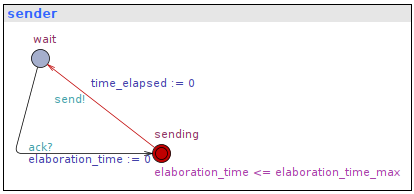
\includegraphics[width=0.8\textwidth]{1_sender.png}\end{center}
Il mittente prepara un messaggio,lo invia un e rimane in attesa di ricevere un Acknowledge, per poterlo inviare si sincronizza sul \channel send (tramite \texttt{send!}) e per riceverlo si sincronizza sul \channel ack (tramite \texttt{ack?}).
Quando un messaggio viene invato viene avviato un timer, \textit{time\_elapsed}, che sarà utile in fase di analisi per stabilire quanto tempo è passato dall'invio del messaggio alla ricezione dell'ack.
\subsection{Destinatario}
\begin{center}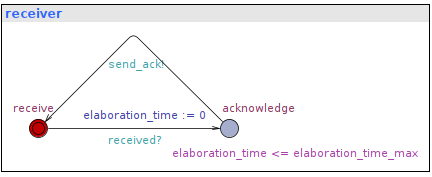
\includegraphics[width=0.8\textwidth]{1_receiver.png}\end{center}
Il destinatario può solo attendere la sincronizzazione sul \channel received, quando il canale gli fornisce un messaggio il Destinatario risponde con un Acknowledge che viene inviato sul canale sincronizzandosi sul \channel send\_ack.
\subsection{Canale}
Il canale presentato è un canale perfetto, quindi riceve un messaggio o un ack e lo consegna senza possibilità di perderlo.
Il canale è half-duplex, quindi permette la trasmissione non simultanea sia da mittente a destinatario che viceversa.\\
\begin{center}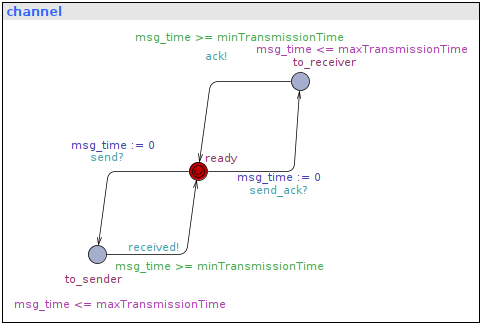
\includegraphics[width=1\textwidth]{channel_safe.png}\end{center}
Il canale quando non sta trasmettendo un messaggio si trova nello stato \textit{ready}, se il messaggio proviene dal mittente il canale si sincronizza sul \channel send e si sposta nello stato \texttt{to\_sender}, da questo stato esce solo dopo \textit{minTransmissionTime} e prima di \textit{maxTransmissionTime}, per rappresentare il tempo di trasmissione varibile del canale.
Per consegnare il messaggio si sincronizza con il Destinatario sul \channel received.\\
discorso diametralmente opposto vare per l'Acknowledge, il canale si sincroniza con il Destinatario sul \channel send\_ack, e consegna l'ack dopo un intervallo di tempo sincronizzandosi con il Mittente sul \channel ack.
In ultimo è presente un timer che viene resettato sull'arco di "presa in carico" di un pacchetto, questo timer può esssere utilizzato per verificare il tempo necessario alla trasmissione di un singolo pacchetto.
\subsection{Analisi}
\begin{itemize}
	\item A[] not deadlock
	\item A[] sender.prepare imply ((time_elapsed >= 2 * minTransmissionTime && time_elapsed <= 2 * maxTransmissionTime) || time_elapsed == 0)
	\item sender.sending --> sender.prepare
	\item sender.sending --> receiver.acknowledge
	\item channel.to_sender --> channel.to_receiver
	\item channel.ready --> (channel.ready && msg_time >= minTransmissionTime && msg_time <= maxTransmissionTime)
	Se parto da uno stato in cui il canale e pronto a trasmettere tornerò dopo qualsiasi esecuzione ad essere pronto a trasmettere dopo un tempo compreso tra maxTrasmissione e minTrasmissione.
\end{itemize}

\section{Modello B}
\section{Modello c}
%controllare anche di non poter spedire il frame 1 senza aver spedito il frame 0
\end{document}
